\documentclass[12pt]{article}
\usepackage[margin=1in]{geometry}
\usepackage{graphicx}
\usepackage{listings}
\usepackage{color}
\usepackage{hyperref}
\usepackage{titlesec}
\usepackage{xcolor}

\titleformat{\section}{\normalfont\Large\bfseries}{\thesection}{1em}{}

\title{\textbf{Digikala Online Shop Simulator}}
\author{Mahla Entezari | Mahla.Entezarii@gmail.com}
\date{April 2023}

\begin{document}

\maketitle

\section{Introduction}
This project is an online shop simulator inspired by platforms such as Digikala and Amazon. It simulates a basic e-commerce experience using Java, JavaFX for GUI, and MySQL for the backend database. It supports functionalities such as user authentication, product browsing, cart and order handling, and comment management.

\section{Technologies Used}
\begin{itemize}
    \item Java (JavaFX)
    \item MySQL
    \item FXML (JavaFX Scene Builder)
    \item MVC (Model-View-Controller) Architecture
\end{itemize}

\section{System Overview}
The system comprises several Java classes that handle different responsibilities:

\begin{itemize}
    \item \textbf{Main.java:} Launches the JavaFX application and initializes the database.
    \item \textbf{ConnectDB.java:} Handles database connection and SQL query execution.
    \item \textbf{DigikalaService.java:} Acts as a backend service for user management, product handling, and login logic.
    \item \textbf{User.java, Admin, Seller:} Represent the user model and its variants.
    \item \textbf{Login.java, Createaccount.java, HelloController.java:} Handle frontend interactions for login, account creation, and navigation.
    \item \textbf{UserPage.java:} Displays categorized product listings and dynamically updates the UI.
\end{itemize}

\section{Database Integration}
A MySQL database is used to store products and user-related data. The application executes queries to fetch products by category and updates the UI accordingly.

\section{Key Functionalities}
\begin{itemize}
    \item \textbf{Login System:} Allows login for three roles – user, admin, and seller.
    \item \textbf{Product Display:} Products are fetched from the database and shown under categories like Mobile, Laptop, TV, etc.
    \item \textbf{Shopping Cart:} Users can add products to their cart and view their orders.
    \item \textbf{Account Management:} Users can register new accounts.
    \item \textbf{Comment System:} Comments are stored in a dedicated table and shown for each product.
\end{itemize}

\section{Challenges Faced}
\begin{itemize}
    \item GUI binding with the backend logic.
    \item Displaying products dynamically in JavaFX components.
    \item Designing a flexible database schema for product comments.
\end{itemize}

\section{Bonus Implementations}
\begin{enumerate}
    \item Graphical User Interface (JavaFX)
    \item Commenting system for products
    \item Search functionality
    \item Persistent data storage via MySQL
    \item Order and sales history
    \item UUIDs for user identification
\end{enumerate}

\section{Sample Code}
Here is an example of database connectivity:
\begin{lstlisting}[language=Java]
public class ConnectDB {
    static private Statement statement;
    public ConnectDB() {
        try {
            Class.forName("com.mysql.cj.jdbc.Driver");
            Connection connection = DriverManager.getConnection(
                "jdbc:mysql://localhost:3306/jdbc", "root", "12345678");
            statement = connection.createStatement();
        } catch (Exception e) {
            e.printStackTrace();
        }
    }
}
\end{lstlisting}

\section{UML Diagram}
\begin{center}
    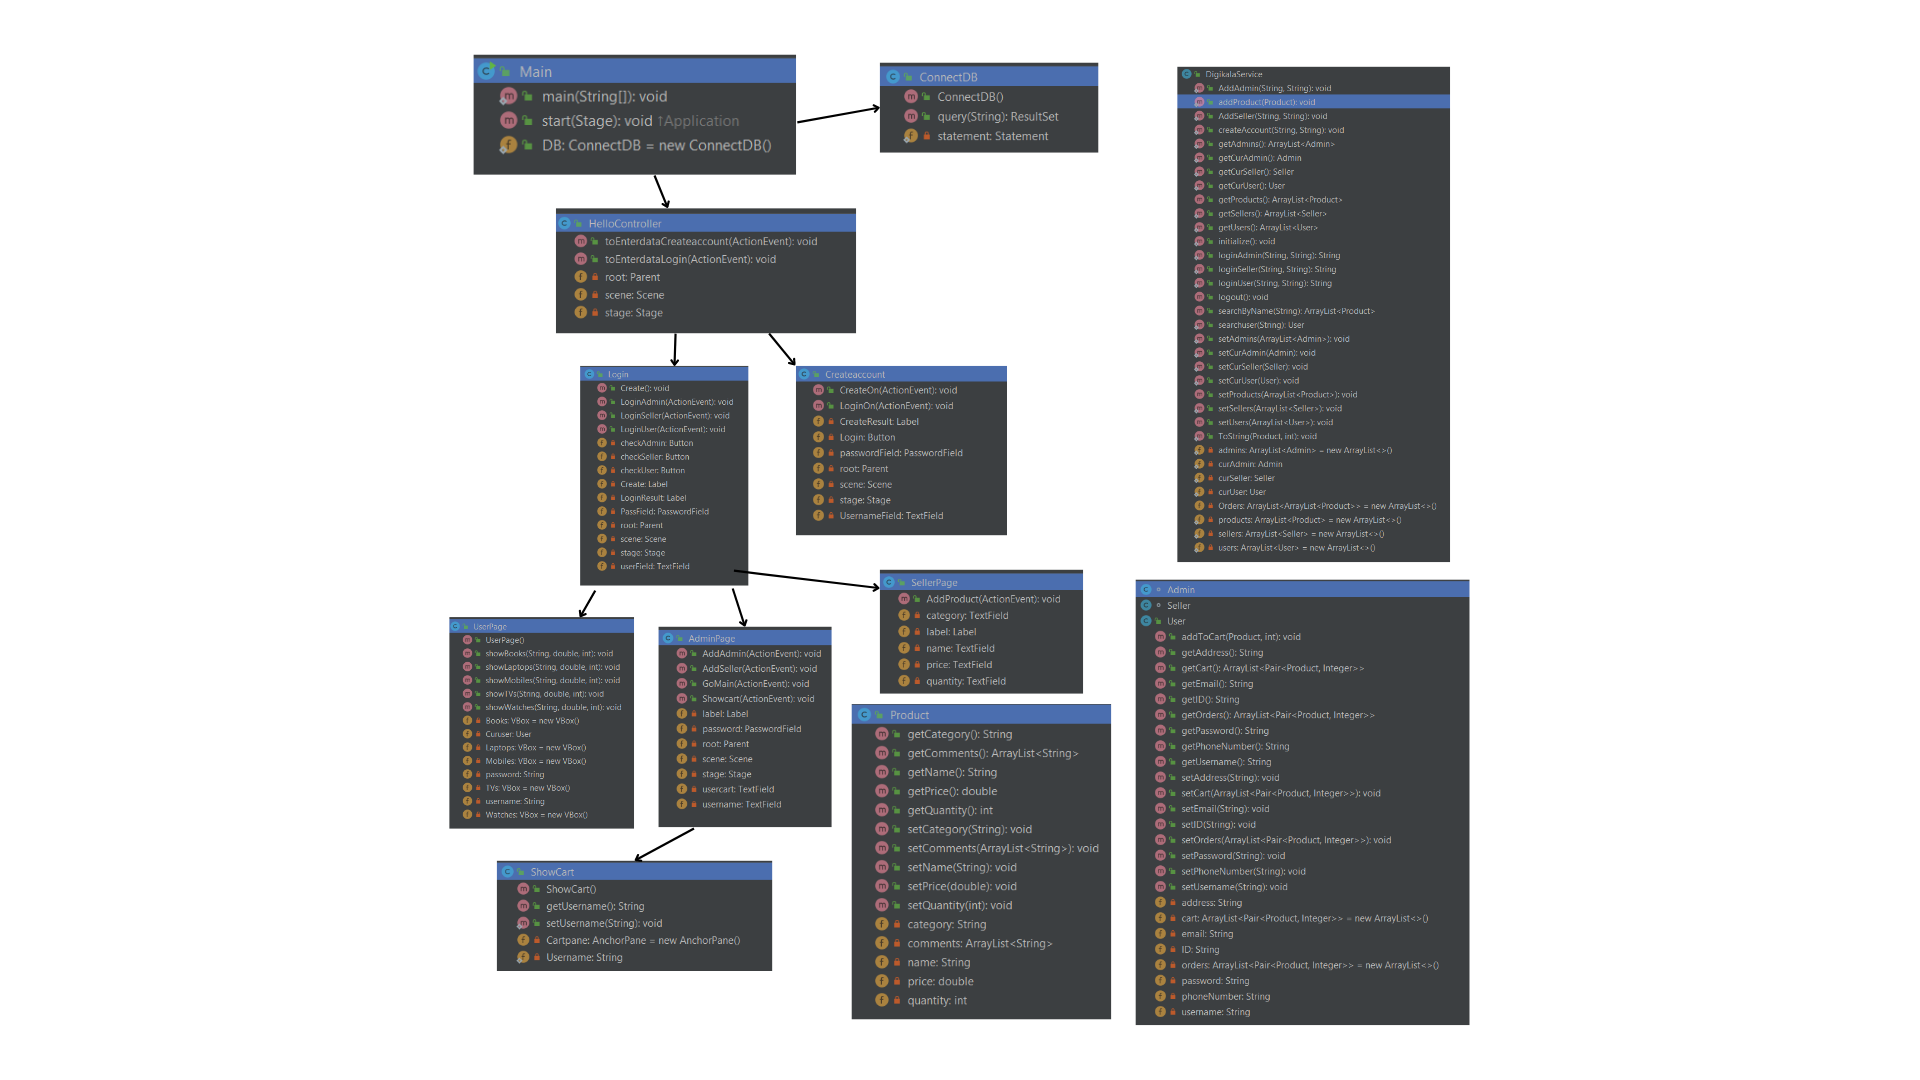
\includegraphics[width=\textwidth]{uml-diagram.png}
\end{center}

\section{Conclusion}
This project successfully simulates a simple online shop system with all necessary modules including user login, product handling, and persistent storage. The integration of JavaFX and MySQL enables a smooth and interactive user experience.

\section{Resources}
\begin{itemize}
    \item \href{https://youtu.be/9XJicRt_FaI}{JavaFX Course}
    \item \href{https://www.youtube.com/watch?v=lz3HilC2bDs&list=PLTfxx5t6obt-fvAmlpoy6bgwFNkBRFSSP&index=1}{MySQL Course}
\end{itemize}

\end{document}
